\section*{Dedicated Security Chips}

Major computing platform providers have recently started to enhance their platforms with new types of dedicated security chips. We look at two examples of this emerging trend: Google’s Titan and Apple’s T2 security chips.

\subsubsection*{Google Titan}

Titan~\cite{titan} is a security chip implemented as a low-power microcontroller on Google’s purpose-built server platforms. The Titan chip communicates with the main CPU via the Serial Peripheral Interface (SPI) and it interposes between the boot firmware flash and system components like the Platform Controller Hub (PCH).

 One of the main functionalities that Titan implements is secure boot. When the server machine is powered up, Titan executes code, known as boot ROM, from its embedded read-only memory. This code is immutable and thus implicitly trusted. The boot ROM code loads Titan’s firmware from the embedded flash memory and verifies its integrity using a digital signature. Once Titan’s own firmware is securely verified and running, it can verify the boot process of its host. Titan blocks PCH’s access to the firmware flash until it has cryptographically verified the content of the flash and then it releases the lock and allows the verified boot firmware to configure the machine and load the boot loader, which subsequently verifies and loads the OS. Such iterative process allows precise control over which version of the system software is booted. 

\begin{figure}[t]
	\centering
	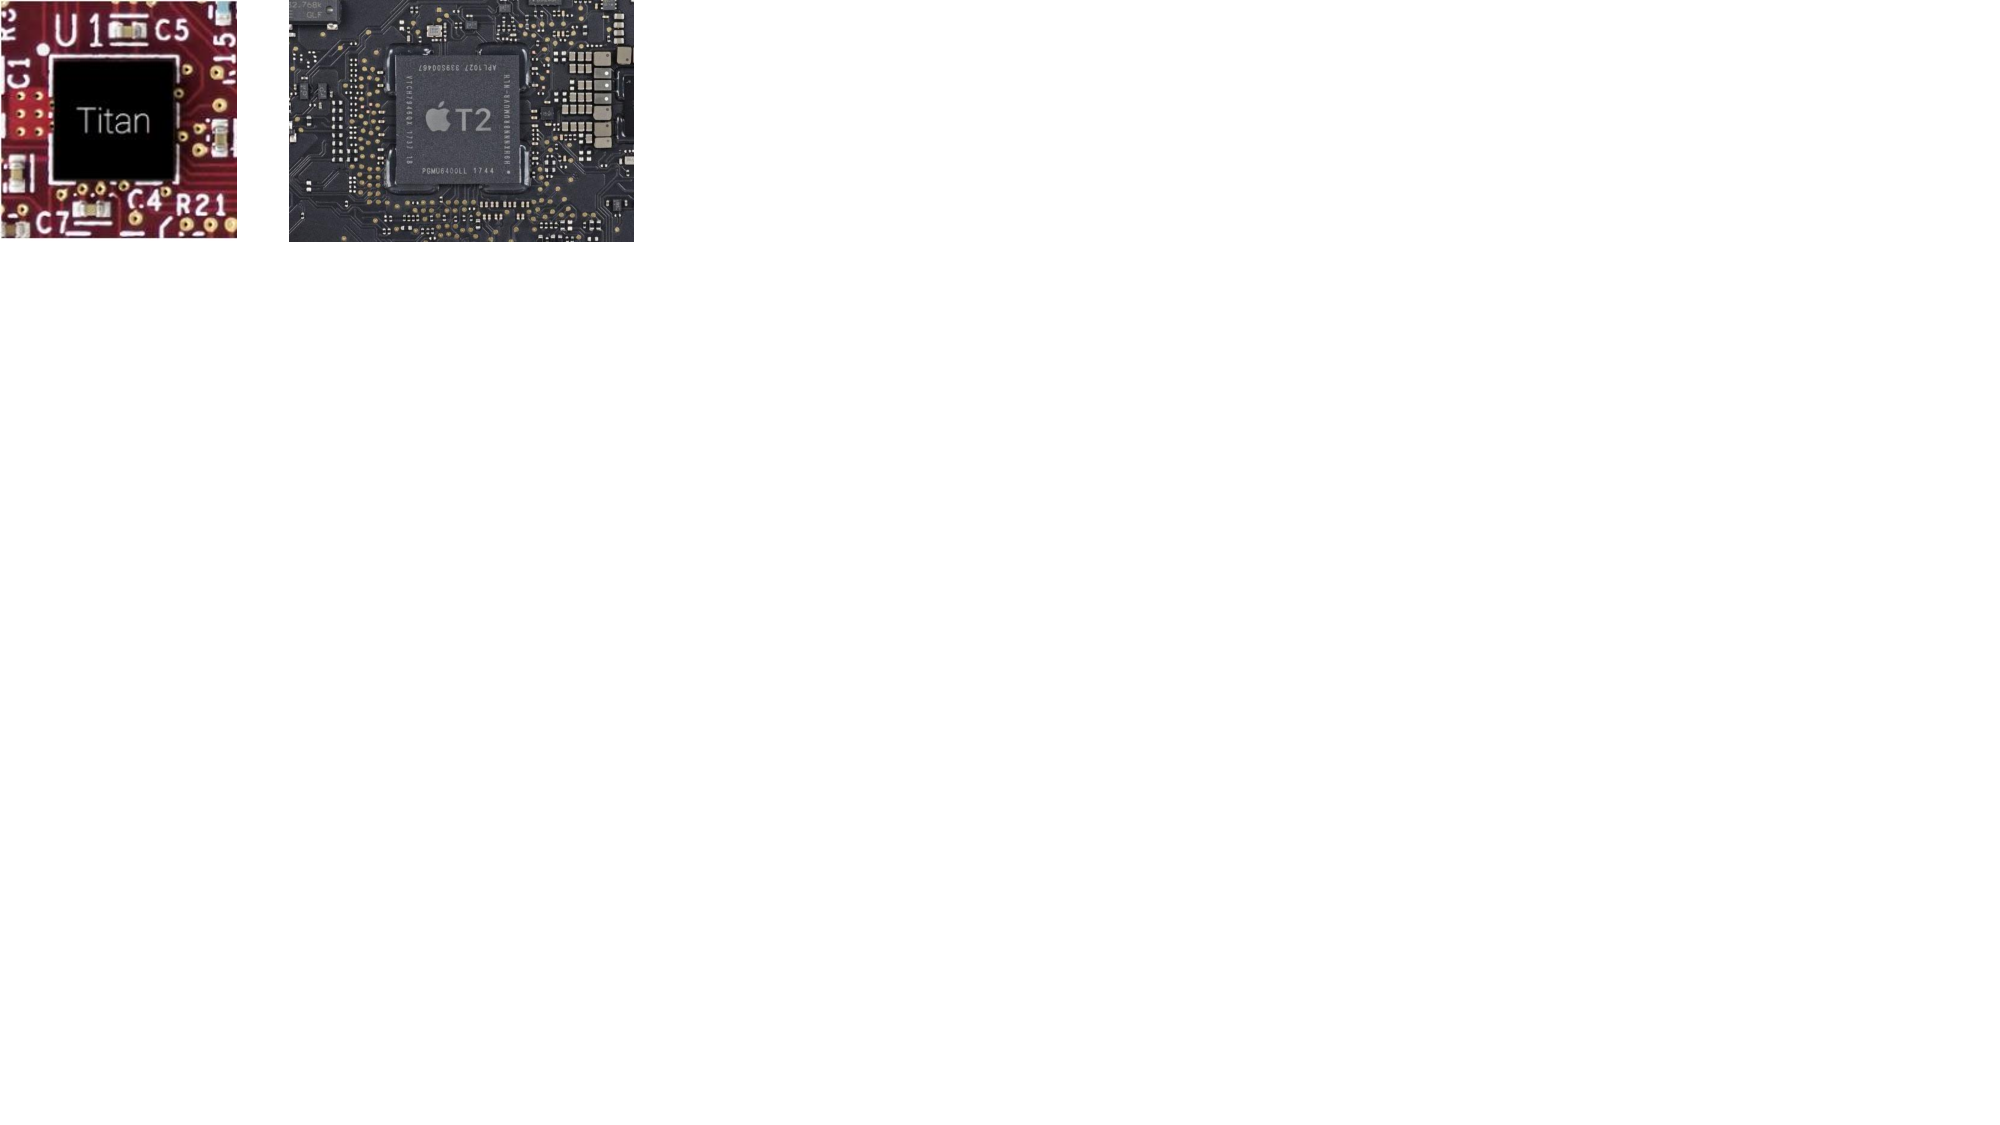
\includegraphics[scale=0.7]{chips.pdf}
	\caption{Dedicated security chips: Google Titan and Apple T2.}
\label{fig:prototype}   
\end{figure}

 
\subsubsection*{Apple T2}
 
 Apple’s latest laptops and desktops come with an integrated security chip called T2~\cite{t2}. Similar to Titan, also T2 enables secure boot. When the machine with T2 chip is turned on, the T2 chip executes code from its read-only memory. This code cryptographically verifies the next step of the T2’s own boot process. Once T2 is fully running it can verify the UEFI firmware which will in turn ensure that only authorized kernel will be booted on the host CPU.

Besides secure boot, T2 provides also other security features such as protecting the user’s fingerprint values or making sure that the microphone is disconnected from the main CPU when the laptop’s lid is closed. 
 
 
\subsubsection*{Missing Functionality}
  
Both Titand and T2 implement secure boot. Secure boot is also a good example of a security mechanism that cannot be implemented using SGX-style enclaves. 

In SGX, and in other similar enclave architectures, enclaves are constructed by the untrusted OS. The construction process of the enclave (i.e., the sequence of setup instructions and their parameters) is recorded by the CPU and can be later communicated to an external verifier using the built-in attestation mechanism. This ensures that secrets will be provisioned only to correctly constructed enclave and thus the OS cannot access those secrets. Thus, SGX enclaves are protected from the OS, but they cannot exist without it. A direct implication of such TEE design is that enclaves cannot verify the integrity of the booted OS. 

As enclaves cannot implement all the needed security services, some platform providers have decided to add dedicated security chips, like Titan and T2, to implement the missing functionality. As noted on Textbox 1, there are also other processor-based TEE architectures like ARM TrustZone that are better suited for secure boot.
%
Disconnecting the microphones from the main CPU is another example of a security feature that, obviously, cannot be implemented using enclaves.
  

\begin{figure}
	\begin{tcolorbox}
	\textbf{Textbox 1:} ARM TrustZone is a processor-based TEE architecture that is commonly used on mobile devices such as smartphones. The main idea of TrustZone is to implement two separate execution modes for the same main CPU. All untrusted software, like the OS and third-party apps, are executed in the normal world mode, while applications that need protection run in a separate execution mode called secure world. The processor and other system components like memory controllers ensure that any process in the normal world cannot access the secure world applications’s memory, and thus modify their execution or read their secrets.

	The TEE design of ARM TrustZone is better suited for the implementation of secure boot~\cite{arbaugh1997secure}. A mobile device can be configured such that when the device is powered up the main CPU starts executing implicitly trusted code that is loaded from a predefined read-only memory location in the secure world mode. This code can then cryptographically verify the normal world boot loader before the CPU starts executing the main boot sequence in the normal world mode. Many current smartphone manufacturers implement such secure boot sequence.
	\end{tcolorbox}
\end{figure}  


\subsubsection*{Security Weaknesses}

Besides missing functionality enclaves have also security weaknesses. Since enclaves and untrusted code share the same CPU, they can be susceptible to side-channel leakage and microarchitectural attacks. The Spectre and Meltdown vulnerabilities showed how transient execution can leak information across isolation boundaries, and the same idea has been applied to extract keys from SGX enclaves in the Foreshadow attack~\cite{van2018foreshadow}. 

While specific attacks can and have been mitigated (for example, Intel’s microcode updates include Spectre and Meltdown patches), side-channel leakage and microarchitectural attacks continue to be a serious concern for enclaves in general. The underlying root cause is the fact that modern processors are extremely complex systems that have been extensively optimized over decades. Enclave support was added on top of many layers of performance optimizations, and now, in hindsight, one can easily say that this approach was not the ideal foundation to realize strong isolation. In this regard, dedicated security chips have a clear advantage over enclaves.

Another security challenge for enclave architectures is the rich interface between the untrusted OS and the protected enclave. Enclaves must interact with the untrusted OS in many ways. For example, enclaves communicate with the rest of the world by sending and receiving messages through the OS. Enclaves also need to safely pause their execution for interrupts, so that the OS can process them. While enclave architectures provide a coarse-grained memory isolation primitive at the hardware level, it is left to the developers to ensure that the interface is well implemented and protected on the software level. Common protective implementation tasks include sanitization of buffers and safety checks of pointers. 

Because such checks can be tedious to implement correctly, several enclave runtimes like Microsoft’s Open Enclave SDK have been developed to assist enclave developers. Unfortunately, recent research has shown that many such enclave runtime have classical memory safety vulnerabilities~\cite{van2019tale}. As dedicated security chips do not need equally extensive interaction with the OS, the interface towards the untrusted OS is easier to protect tightly. 


\subsubsection*{Other Security Services}

To summarize our discussion so far, enclaves cannot implement all useful platform security mechanisms and they also have significant security limitations. Dedicated security chips can address both of these concerns. 

Obviously, the possible security mechanisms that dedicated security chips can provide is not limited to previously discussed examples like secure boot and disconnecting peripherals. Which other security mechanisms are missing from modern enclave-supporting computing architectures? And how should such security mechanisms be implemented as special-purpose security chips? Titan and T2 are integrated security chips. Are there use cases that would benefit from external and plug-and-play security tokens?

In the rest of this article, we explore these questions by examining two case studies from our recent research. Our first case study is the implementation of trusted path using a low-complexity hardware security module. After that we explain how secure TEE identification can be realized using a simple user-pluggable security token.
